\section{An Image's Odyssey through the System}

To summarize the previous sections, let us take a quick example on how the
complete system will process a video, an image or something like the Game of
Life.

At first, the machine is powered up, and all the components wake up from their
sleep. \ac{LENA} will reload its \ac{FPGA} setup from flash, and the \ac{SCU}
will do the same. When these are ready to run, the \ac{SCU} creates a menu and
sends it to \ac{LENA}, which will in turn show the menu trough the \ac{VGA} port
it has control over. Whenever a user push any of the buttons, the menu is
updated and a new menu image is sent over to \ac{LENA}.

When we have chosen the program to run and the data it should run on, the
\ac{SCU} sets the \ac{LENA} state to a state where it is able to receive
instructions. It then loads the instructions the program contains to
\ac{LENA}. The \ac{SCU} then sets the state to a state where it is able to load
data, and loads the data. Finally, the \ac{SCU} allows \ac{LENA} to run. The
  \ac{SCU} will feed \ac{LENA} with more data after some time, depending on what
  data stream we have chosen and what program we have decided to run.

\begin{figure}[h]
  \centering
  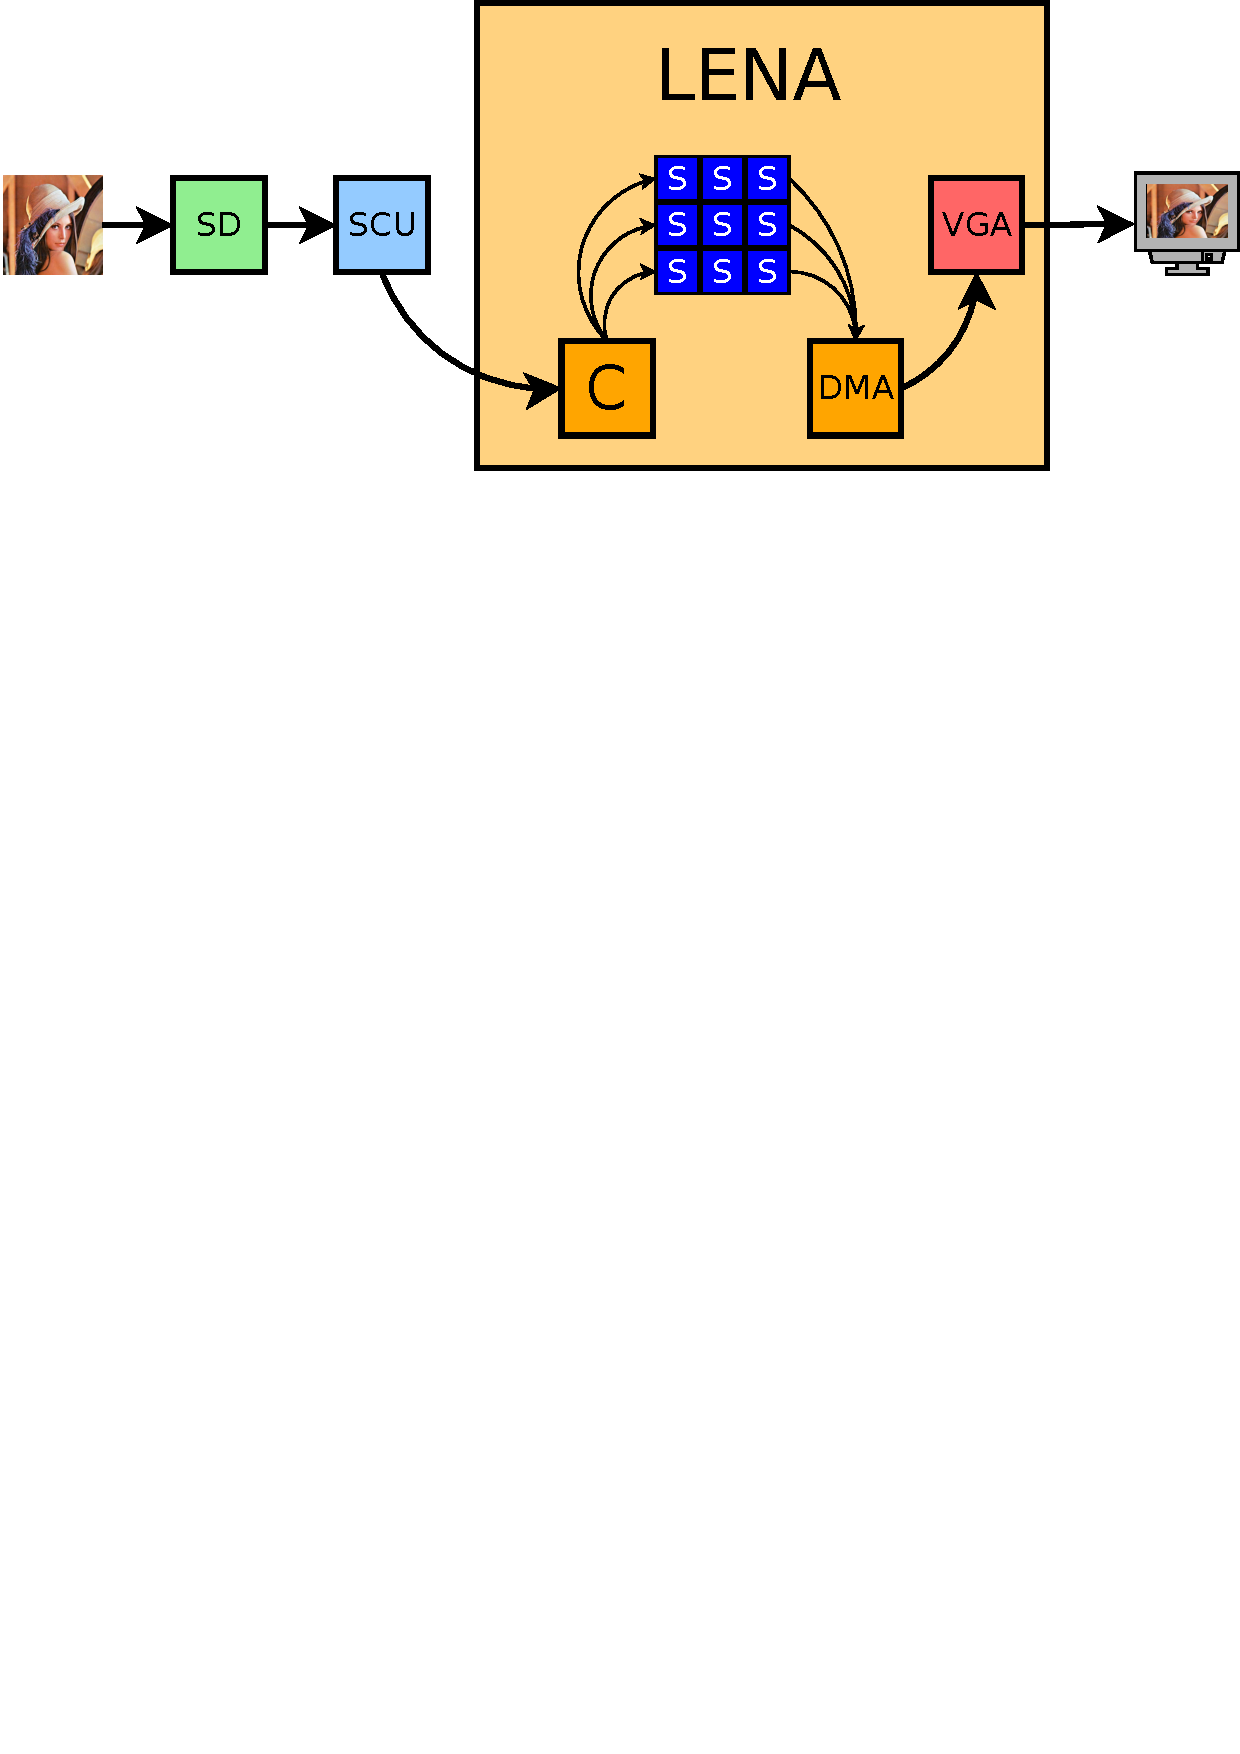
\includegraphics[width=\linewidth,clip,trim=0 21.5cm 0 0]
                  {fig/sys-over/journey.pdf}
  \caption{The Journey of an Image}
  \label{fig:image-journey}
\end{figure}


\ac{LENA} has now all it needs to perform its instructions. The control core
starts by activating the \ac{DMA}. The \ac{DMA} starts sending data from memory
to the \ac{SIMD} array. This is done by putting the different values on multiple
``conveyor belts'' which lies below the \ac{SIMD} node. \TODO{This is very
  illustrative, but not technically correct. Is that an issue?} When every
\ac{SIMD} node has data to work with, every node ``picks up'' the data and
places it in a special register.

The control core then sends the instruction the \ac{SIMD} nodes should use
next. In parallel, the \ac{DMA} starts sending in new data into the \ac{SIMD}
nodes, to minimize latency. When the \ac{SIMD} nodes have finished processing
this data, they swap the finished result with the new data on the ``conveyor
belt''. The \ac{DMA} puts on new data, and the finished results are moved on and
out of the ``conveyor belt''. The \ac{DMA} takes the finished result and puts it
back into the data memory.

The control core then takes the results from memory and sends them to the
\ac{VGA} module, which finally sends the image to the device connected to the
\ac{VGA} port. The device, a screen, for instance, then displays the processed
image.

The odyssey has ended for our image, but there is still work to be done. If we
are playing a video, more images will be processed in the way described
above. If we are doing something entirely different | for instance, playing Game
of Life | we may just keep working on the result from last iteration until the
end of time. If we stop before that, the \ac{SCU} will stop \ac{LENA} by turning
its state to a stop state. The \ac{SCU} will then set up the original menu, and
our machine is ready to let new images go on another odyssey with another
program.
